\documentclass{article}
\usepackage{hyperref}
\usepackage{tikz}
\usepackage{python}
\usepackage[%
    natbib=true,%
    backend=biber,%
    backref=true,%
    citestyle=authoryear-comp,%
    bibstyle=authoryear,%
    maxbibnames=24,%
    maxcitenames=2,%
]{biblatex}

\hypersetup{%
    bookmarks=true,
    colorlinks=true,
    pdfauthor={Luis Pedro Coelho},
    citecolor=pondgreen,
    urlcolor=toastedchilipowder,
    linkcolor=toastedchilipowder,
}
\let\code\texttt

\title{Jug: Software for Reproducible Computation}
\author{Luis Pedro Coelho}

\begin{document}
\section*{Abstract}
As computational pipelines become a bigger part of science, it is important to
ensure that the results are reproducible. All developed software should be able
to be run automatically without any user intervention.

In addition to the value to the community of being able to reproduce an
analysis, reproducible research practices allow for better control over the
project. For example, if necessary parameters to run a pipeline are kept
separately from the code that implements it (perhaps even in the researcher's
mind), this leads to error-prone analysis and opens up the possibility that
when the results are to be writtne up for publication, the researcher will no
longer be able to even completely describe the process that led to them.

For large projects, the use of multiple processors (either in the same machine
or distributed across a cluster) is necessary to obtain results in a useful
timeframe. Furthermore, it is often the case that, as the project evolves, it
becomes necessary to save intermediate results while down-stream analyses are
designed (or redesigned) and implemented. Therefore, having a single point of
entry (often in the form of a single script or a single main programme) for the
computation becomes increasingly difficult.

Jug is a software framework which solves all of these problems in a
simple way. Jug supports caching of intermediate results, distribution of
computation as tasks across a network.

Jug is written in pure Python, is completely cross-platform, and available as
free software under the MIT license. Jug is available from
\url{http://github.com/luispedro/jug}.

\section{Introduction}
Jug is a task-based framework for Python, which supports saving and sharing of
intermediate results and parallelisation on computer clusters (or multi-core
machines).

By allowing caching of results, where the caching depends explicitly on the
input parameters of that computation. Any change in the parameters immediately
triggers a recomputation of all dependendent results. The basic model is
similar to the one of the venerable Unix tool Make~\citep{}, which has been
used before for implementing reproducible research pipelines~\citep{}.

However, unlike make, jug is written in Python and tasks can consist of any
Python function and its arguments. A jugfile (the file which specifies which
tasks need to be run---named by analogy to the makefiles of make) is a simple
Python script with some added notations (we will see just how little changes
need to be made from a conventional Python script).

\section{Design Choices}
\subsection{Task Based Architecture}

Jug is designed around tasks. A task is defined as a Python function and a set
of arguments, which may be Python values or the output of other tasks. A task
should be a pure function, but there is no way of mandating this in the
language.

\begin{python}
from jug import Task

def count(imname):
    ...
    return value

def mean(args):
    return sum(args)/float(len(args))

images = glob('*.png')
counts = [Task(count, im) for im in images]
final = Task(mean, counts)
\end{python}

\begin{figure}
\begin{center}
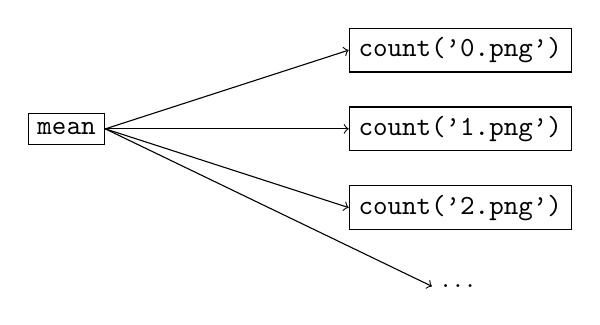
\begin{tikzpicture}
\node (mean) at (0,2) [draw] {\code{mean}};
\node (count0) at (5,3) [draw] {\code{count('0.png')}};
\node (count1) at (5,2) [draw] {\code{count('1.png')}};
\node (count2) at (5,1) [draw] {\code{count('2.png')}};
\node (countn) at (5,0) {\ldots};

\draw[->] (mean.east) -- (count0.west);
\draw[->] (mean.east) -- (count1.west);
\draw[->] (mean.east) -- (count2.west);
\draw[->] (mean.east) -- (countn.west);
\end{tikzpicture}

\end{center}
\caption{Simple Dependency Structure for Example in the Text. This assumes that
the directory had a collection of images names 0.png, 1.png,\ldots}
\label{fig:jug-deps}
\end{figure}

This defines the task dependency structure represented in
Figure~\ref{fig:jug-deps}. As we can see, all of the \code{count} operations
can be run in parallel, while the \code{mean} operation must wait the result of
all of the other computation. The dependency structure is always a \textsc{dag}
(directed acyclic graph). Only by bypassing the normal use mechanisms is it
even possible to construct a cycle.

The code above has the construct \code{Task(f, args)} repeated several times.
Using the decorator \code{TaskGenerator} decorator this can be simplified to a
more natural syntax.

\begin{python}
from jug import TaskGenerator

@TaskGenerator
def count(imname):
    ...
    return value

@TaskGenerator
def mean(args):
    return sum(args)/float(len(args))

images = glob('*.png')
counts = map(count, images)
final = mean(counts)
\end{python}

As the reader can appreciate, this is identical to a traditional Python script,
except for the \code{@TaskGenerator} decorators. With a few limitations (which
unfortunately can give rise to complex error messages), scripts can be written
as if they were sequential Python scripts.

By default, jug looks for a file called \code{jugfile.py}, but any filename can
be used. Generically, we refer to the script being run as the jugfile.

\subsection{Jug subcommands}

Jug is structured as a series of subcommands, the most important of which are
\emph{execute}, \emph{status}, and \emph{shell}.

Execution is the command used for running the tasks. In broad terms it performs
the loop below.

\begin{python}
tasks = alltasks in topological sort order
while tasks:
    next = task.pop()
    if not next.has_run() and not next.is_running():
        while not next.can_run():
            wait a while
        with locked(next):
            next.run()
\end{python}

If run on a single processor, this will just run all of the tasks in order. It
is most interesting when it is run on multiple processors. There it executes
all of the tasks that can be executed in parallel.

Of course, the actual code is more complex than what is shown above,
particularly to make sure that the locking is performed correctly and that the
waiting step eventually times out (in order to handle the situation where
another process is hung).

\begin{figure}
\begin{verbatim}
$jug status images.py
Task name         Waiting      Ready   Finished    Running
----------------------------------------------------------
images.mean             1          0          0          0
images.count            0         20          0          0
..........................................................
Total:                  1         20          0          0
\end{verbatim}
\caption{Output of \code{jug status}. The \texttt{\$} sign shown is the command
line prompt, and the status subcommand was run. At this point, nothing has been
run. The output has been edited for space reasons (spacing columns were
removed).}
\label{fig:jug-status-output}
\end{figure}

The status command prints out a summary of the status of all of the tasks.
Figure~\ref{fig:jug-status-output} shows the output of this command using the
example jugfile above. We assume that the jugfile was called \code{images.py}
on disk and that there were 20~images in the directory. We can see that there
are 20~tasks ready to run, while the \code{mean} task is still waiting for the
results of the other tasks.
\subsection{Backends}

A basic feature of jug is its ability to save and load results. Each task
\code{Task(f, args)} is represented by a hash of \code{f} and \code{args} in a
way that uniquely identifies it.

A jug backend must then support four basic operations:

\begin{description}
\item[save] Saving a Python object by its hash name.
\item[load] Loading a Python object by its hash name.
\item[lock] Creating a lock by hash name. Naturally, this lock must be created
atomically.
\item[release] Releasing the lock.
\end{description}

A few other operations, such as deletion and listing of names are also
supported.

The filesystem can support all of the above operations if the backend is coded
correctly to avoid race conditions. This is the default backend, identified
simply by a directory name. Inside this directory, files named by a hexadecimal
representation of their hashes. Objects are saved using Python's \code{pickle}
module with zlib compression. As a special case, \code{numpy} arrays
\citep{numpy} are saved to disk directly. For functionality, there was no need
for this inelegant special case as \code{numpy} can be saved as a pickle dump,
but \code{numpy} arrays are a very common data type in scientific programming
and saving them directly allows for very fast saving and loading (they are
represented on disk as a header followed by the binary information they
contain).

Another backend currently included with jug is a redis backend. Redis a
name-key database system.\footnote{See the redis webpage, at
\href{http://redis.io}{redis.io}, for detailed information about redis.} Redis
is particularly recommended for the case where there are many small objects
being saved. In this case, keeping each as a separate file on disk would incur
a large space penalty, while redis keeps them all in the same file.

Finally, there is an in-memory backend. This was initially developed for
testing, but can be useful on its own.

\subsection{Asynchronous Function}

Parallelisation is achieved by running more than one jug process
simmultaneously. All of the synchronisation is outsourced to the backend. This
has certain limitations, but it makes jug usable in cluster computing
environments with a batch architecture. As long as all of the processes can
access the backend, there is no need for them to communicate directly.
Therefore, it can even be the case that processors start working on tasks in
mid-processing.

\subsection{Development Support}


The output of computation can be obtained from jug in two ways: (1) One can
simply write a task that outputs the desired format. (2) They can be inspected
interactively using the \emph{shell} subcommand. It is expected that the first
option will be used for the final version of the computation, whilst the second
one is most helpful during development.

The shell subcommand, invokes an IPython instance with all the objects in the
jugfile loaded. IPython is an enhanced interactive shell for Python
\citep{Perez2007}. A few functions are added to the namespace, in particular,
\code{value} can load the results of a task object if necessary.

\begin{figure}
\begin{center}
\begin{verbatim}
$jug shell images.py

=========
Jug Shell
=========


Available jug functions:
    - value() : loads a specific object
    - load_all() : loads all objects

Enjoy...


In [1]: value(final)
Out[1]: 7.5

In [2]: value(counts)
Out[2]: [7, 7, 7, 7, 7, 7, 7, 7, 7, 7, 8, 8, 8, 8, 8, 8, 8, 8, 8, 8]
\end{verbatim}
\end{center}
\caption{Interaction with \code{jug shell}.}
\label{fig:jug-shell-interaction}
\end{figure}

Figure~\ref{fig:jug-shell-interaction} shows a possible interaction session
with jug shell. While having to explicitly load all the results is a bit
bothersome, it has some advantages versus the alternative of pre-loading all.
It is much faster at startup. Consider too that the user might not load more
than a few objects. In some cases, loading all of the objects simultaneously
might even be impossible due to memory constraints. Further, this allows
exploration of the task structure for debugging.

\subsection{Result Invalidation}

It is often the case that one improves a step in a computational pipeline and
wished to obtain the result of recomputing the pipeline while reusing as much
of the previously computed intermediate results. With the manual management of
results I found this to be the most error-prone operation: by not removing
enough of the intermediate files, it was easy to generate an irreproducible
state where part of the computations were made using one version of the code
and part with another.

Therefore, jug adds some support for result invalidation. When a results from a
task are invalidated, all tasks which, directly or indirectly, depend on them
are also marked for deletion.

It is still necessary to manually invalidate tasks. An alternative, which I
considered, was to have the code which implements the task be taken into
account while computing the hash. While this would add another layer of
protection, it would still be possible to make mistakes. If the function
depended on other functions, especially if this was done in a dynamic way, it
could be hard to discover all dependencies (cf.\ sumatra~\citep{sumatra}).
Additionally, minute refactoring of the code would lead to over eager
recomputation. This could make the developer wary of making improvements in
their code, resulting in overall worse code.

Therefore, I chose to force the user to explicitly invalidate his results,
while supporting automatic dependency discovery to make it easier for the user.

\section{Methods}
\section{Example}
I will present an example from my research. Although it introduces some
unnecessary complexity, it has the advantage of being a real-life example of
the usage of jug.

The goal of this project was to demonstrate that using local features, in
particular speeded-up robust features (henceforth,
\textsc{surf})~\cite{surf-paper} improves over image-global features for
classification of microscope images. A variation of standard \textsc{surf},
\textsc{surf}-ref, was introduced and tested.

To evaluate classification, the dataset is broken up into 10~pieces and each of
the pieces is held-out of the analysis and then used to evaluate analysis (the
final result is the average of all ten values). This is known as
cross-validation. In this case, I use another library (which I also wrote)
which has a builtin method for jug-aware cross-validation.

\begin{python}
from jug import TaskGenerator, CachedFunction

# pyslic is used for subcellular location analysis
import pyslic

# milk (machine learning toolkit)
from milk.ext.jugparallel import nfoldcrossvalidation

datasets = [ 'data0', 'data1', ]
featuresets = [ 'field-dna+', 'surf', 'surf-ref', ]

def load(dset):
    '''
    This function assumes that the images are stored in ../data/dset with
    filenames matching the pattern
    label-(protein|dna)-([0-9]).tiff
    '''
    from os import listdir
    images = []
    base = '../data/'+dset
    for path in listdir(base):
        if not 'protein' in path: continue
        label = path.split('-')[0]
        # We only store paths and will load data on demand
        # This save memory.
        im = pyslic.Image({
                'protein': base + path,
                'dna' : base + path.replace('protein','dna')
                })
        im.label = label
        images.append(im)
    return images

# pyslic.computefeatures takes an image and an identifier of the feature set
# and returns a set of features (as a numeric array).
#
# TaskGenerator can be used directly to adapt existing functions
computefeatures = TaskGenerator(pyslic.computefeatures)

# or it can be used as a decorator on a newly defined function
@TaskGenerator
def output(cmatrix, dset, fset):
    output = file('results/cmatrix-'+dset+'-'+fset+'.txt', 'w')
    print >>output, cmatrix
    output.close()

features = []
for dset in datasets:
    images = CachedFunction(load, dset)
    labels = [im.label for im in images]
    for fset in featuresets:
        features = [computefeatures(im, fset) for im in images]
        cmatrix = nfoldcrossvalidation(features, labels)
        output(cmatrix, dset, fset)
\end{python}

\section{Development of Jug}
Jug is available under the MIT software license, which grants the user right to
use, copy, and modify the code almost at will. It is developed using the git
version control tool, with the project being hosted on the github
platform.\footnote{The jug project is available at
\url{https://www.github.com/luispedro/jug}.} An open mailing-list provides
support and reported bugs are generally fixed within hours.

Jug includes a full test suite. There are no known bugs.

Jug has been available in the Python Package Index\footnote{The Python Package
Index, PyPI, is accessible at \url{http://pypi.python.org}.} since May~2009
and has been downloaded over 6000~times (some of these downloads may, of
course, represent upgrades, and users which downloaded it from some other
source will not be counted).% FIXME: Check download number. At 5713 8/31/2011

\section{Discussion}
Unlike most previous tools for reproducible research, jug focuses on the
development of the computation as much as its communication (in fact, when it
comes to communication other tools might be better targetted as they combine
written exposition with computer code). While it still possible to make errors
(for example, by changing the code but neglecting to invalidate the results),
jug improves the pipeline development experience and makes the programming
researcher more productive.

In the last few years, I have not undertaken any computational research project
without the use of jug to manage my computations. The tool has become an
indispensible part of my toolkit.

\end{document}
